%\chapter[简明数学史]{智能，生于数学}
\chapterwithsubtitle{智能，生于数学}{简明数学史}

\begin{introduction}
\item Definition of Theorem
\item Ask for help
\item Optimization Problem
\item Property of Cauchy Series
\item Angle of Corner
\end{introduction}

“如果人们不相信数学很简单，那是因为他们没有意识到生活有多复杂。”
\begin{flushright}
约翰·冯·诺伊曼
\end{flushright}

“课本中字斟句酌的叙述，未能表现出创造过程中的斗争、挫折，以及在建立一个可观的结构之前，数学家所经历的艰苦漫长的道路。学生一旦认识到这一点，他将不仅获得真知灼见，还将获得顽强地追究他所攻问题的勇气，并且不会因为自己的工作并非完美无缺而感到颓丧，实在说，叙述数学家如何跌跤，如何在迷雾中摸索前进，并且如何零零碎碎地得到他们的成果，应使搞研究工作的任一新手鼓起勇气。  ”
\begin{flushright}
                                                 克莱因，《古今数学思想》序言
\end{flushright}

智能的历史可以追溯到人类最早期的思维活动，而数学是其中最重要的基础工具之一。

对于古代人来说，数字的发明源于对数量的需求。无论是借助手指计数，还是用其他物体辅助，人类通过千年的发展，逐渐完善了从简单符号到抽象数字的演变过程。今天，我们的“自然数”概念似乎理所当然，但这一切都建立在人类历史上无数次的试错与进化中。

人类对“智能”的探讨源远流长。远在古希腊时期，哲学家们就已经开始追问：什么是智慧？什么是理性？我们如何通过思维去理解这个世界？从那时起，人们就梦想着创造能自主思考的机器。神话人物皮格马利翁(Pygmalion)、代达罗斯(Daedalus)和赫淮斯托斯(Hephaestus)可以被看作传说中的发明家，而加拉蒂亚(Galatea)、塔洛斯(Talos)和潘多拉(Pandora)则可以被视为人造生命(OvidandMartin,2004;Sparkes,1996;Tandy,1997)。

这些问题不仅关乎哲学，还对现代科学和技术的发展产生了深远影响。随着时间推移，这种对智能的追问从哲学的纯理论思辨，逐渐转向了科学与工程的实践领域。

早期的数学家如欧几里得、阿基米德以及笛卡尔等，通过逻辑和结构化的思维方式，奠定了后来发展计算机智能的理论基础。他们的工作不仅推动了科学与工程的发展，也为智能的理论构建提供了明确的框架。

数学的发展历程如同一条不断延展的长河，从最初的数字发明，到公元前5世纪的希腊数学奠基，再到随后的数千年中，数学逐渐演变为一门多维度、多分支的科学。通过计算与推理的结合，数学不仅成为解决现实问题的工具，也升华为探索抽象概念与逻辑关系的强大思维体系。

数学的发展史可以大致划分为四个不同的时期：数学萌芽时期、初等数学时期、近代数学时期和现代数学时期。需要说明的是，精确地划分这些阶段是不可能的，因为每个时期的特征都是在前一时期的基础上逐渐形成的。然而，这些阶段反映了数学在每个历史阶段中的不同侧重与进步，揭示了数学从最早的经验积累到复杂的理论构建，乃至今天在科技与智能领域的广泛应用的深刻演化。每个时期都在数学发展中扮演了不可或缺的角色。

让我们依次回顾这些数学发展的重要阶段，探索其背后的历史背景与核心成就。

\section{数学萌芽时期}
数学的萌芽时期从远古时代延续至公元前5世纪，是人类最早利用数学工具应对日常生活需求的阶段。

这一阶段的数学起源于最基本的数数活动。通过手指计数、刻痕和结绳等原始计数手段，人类逐渐形成了自然数的概念。自然数的确立是数学发展的第一步，也是人类对数量的最早认识。从简单的数数开始，逐渐发展出加减乘除等基本运算，为解决日常生活中的问题提供了有效的工具。

古埃及人发展了一些基础的几何公式，在建造金字塔时已经能够运用高度和角度的几何关系；美索不达米亚的会计师不仅掌握了加法和乘法，还能够解简单的二次方程，用于管理粮食和资源。古代美索不达米亚和埃及的泥板和石刻记录了这些早期的数学活动，展现了数学与生活实践的紧密联系。

巴比伦人对天体运动的观察和历法推算也推动了数学的发展。为了精确预测日食、月相以及制定历法，巴比伦的天文学家需要处理大量的时间和角度计算。这些天文观测不仅促进了数学在测量和计算方面的进步，也推动了几何和代数的进一步发展。

这一时期并没有明确的个人数学家记载，更多的是群体性活动。古埃及的建筑师和美索不达米亚的会计师是这一阶段数学发展的重要推动者。埃及人在几何测量中的应用和美索不达米亚人对天文学和代数的研究，构成了数学早期发展的代表性成就。

这一阶段的数学活动是解决问题的经验性工具，尚未形成系统的理论。但它为后续的数学体系发展奠定了数与形的概念基础。

%\section{数字的发明，智能的开端}
\subsection{史前数学：日常需求与实用计算}
数学史往往是从公元前5世纪的希腊开始讲起的。毕达哥拉斯创立了算术，泰勒斯和阿那克西曼德创立了几何，奠定了古代数学的两大分支。算术和几何的创立，无疑是数学史上的重大突破。然而，这样的讲法却忽略了一个重要的时代，也就是所谓的“史前”数学。人们并没有等到公元前5世纪才开始解决数学问题，特别是那些日常面临的具体数学问题。

在公元前5世纪之前，数学并非一种独立的学科，而是伴随着人类生活的需要而逐步发展起来的。史前数学的主要任务是应对日常生活中的具体问题，如计数牲畜、测量土地和管理时间。远古人类通过手指计数、刻痕和结绳的方式解决了基本的数量和度量问题，虽然这些方法原始，却为后来的数学奠定了基础。

人类早期的数学成就源于实际需求，古埃及人和巴比伦人便是典型的例子。他们在天文学、土地测量和贸易中依赖数学工具，通过经验性的方法逐渐累积了丰富的数学知识。然而，这些方法主要依赖于实用性，而非系统的理论研究。

“数学”活动最古老的痕迹之一是在美索不达米亚发现的一块泥板，它可以追溯到公元前2500年。这块泥板记录了这样一个计算:如果一个谷仓里有1152000份粮食，每个人分得7份，一共可以分给多少人呢?不出所料，结果是164571人，即用1152000除以7得到的结果。看来，美索不达米亚的会计师在算术“诞生”之前很久就知道怎么做除法了。甚至，书写完全有可能就是为了记账才发明的——虽然这些事情很难说得准，但若真是如此，数字就比字母发明得还要早了。

\subsection{手指：长在身上的计数器}
相信你在许多影视剧中都见过这样的一幕：一位算命先生，掐指一算，口中念念有词。这种“掐指一算”看似神秘，实则源自于古老而简便的计数方法。
\begin{figure}[htbp]
\centering
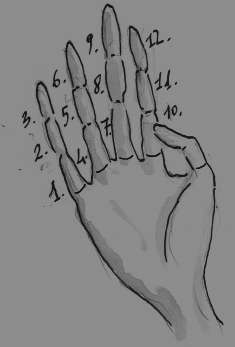
\includegraphics[width=0.3\textwidth]{figs/fingers.png}
\caption{“掐指一算”}
%\label{}
\end{figure}

在远古时代，用手指计数是再自然不过的选择，手指是人类最早的“随身计算器”。手指提供了一个天然的计数系统，帮助人们轻松应对日常的计数需求，如记录牲畜数量、物品交换量，推算季节、节气，安排农耕节日等活动。

%%\subsection{手指计数与各种进制系统}
手指的构造与多种进制系统有着天然的联系。稍加思考，我们就可以发现十进制、二十进制、十二进制等计数法与手指构造的对应关系。

十进制(Decimal System)是最常见、最自然的计数方式。双手的十根手指与十进制自然对应，每根手指代表一个数字，从1数到10，完成一轮计数。十进制系统在全球的广泛使用，源于人类天生拥有十根手指的解剖学特征。正如爱德华·卢卡斯所言，这是“自然界的一个偶然事件”​。

十二进制(Duodecimal System)则适用于更复杂的计数需求。除大拇指外，四根手指各有三段指节。一只手的大拇指指向四根手指的各段指节，可以计数1到12。这种方式在古代美索不达米亚和古埃及广泛应用，至今仍用于时间和角度的计数系统中，如12小时制、一年12个月等。

六十进制(Sexagesimal System)则更加复杂。它结合双手来计数。一只手用于计12（与十二进制相同），另一只手的五根手指则记录12的倍数，五轮12等于60。六十进制在古巴比伦时期被发明，沿用至今，广泛用于时间和角度的计量，例如1小时=60分钟，1分钟=60秒，以及360度的圆周划分。

二十进制(Vigesimal System)也是一种古老的计数法。为了更大范围的计算，一些古代民族不仅用手指，还加上脚趾来计数。例如，中美洲的玛雅文明和阿兹特克文明，以及现今的西非和欧洲部分地区，采用了以20为基数的计数法。

二十进制的痕迹在许多语言中依然存在。现代英语中的"score"表示20的用法便保留了这一印记。例如，莎士比亚在《圣经》英译本中使用“three score and ten”（20的3倍加10，表示70岁)来指代古稀之年；林肯在《葛底斯堡演讲》中使用“four score and seven years ago”(20的4倍加7，表示87)来表达87年前的历史。一百年后，马丁·路德·金在其著名的演讲《I have a dream》中说“Five score years ago”​（20的5倍，即100年前）​。如今，在现代英语中，“score”的这种用法已不再常见。

英国曾有一个结合十二进制和二十进制的货币系统：1英镑=20先令，1先令=12便士。1971年，英国引入了十进制货币系统，1英镑=100便士，先令在1990年后彻底退出流通。

在法语、丹麦语和巴斯克语中也能找到二十进制的痕迹。例如，法语中的数词从quatre-vingts(80)​、quatre-vingts-dix(90)​，到quatre-vingts-dix-neuf(99)，表明凯尔特族过去采用二十进制计数法。同时，这些语言中还混杂了六十进制的痕迹，如数词soixante(60)到soixante-dix-neuf(79)。

手指不仅是我们身体的一部分，还是人类最早的天然计算工具。它帮助我们理解和组织世界，并为现代数学中的位值制和进制系统提供了最初的灵感。直到今天，手指仍是许多人在进行简单计算时的本能工具。可以说，手指是人类最早的“计算器”，引领我们从最原始的计数方法走向了复杂的数学世界。

\subsection*{自然的教育，数字文明的缩影}
设想你在一次航海探险中遭遇风暴，不幸漂流到了一个无人孤岛。没有手表、手机，也没有任何现代工具。你很快面临一个问题——如何计算时间？如何记录每天收集的食物？在这种完全回归自然的环境中，你必须依靠最原始的方式来解决这些问题。

\subsection*{手指计数：最简单的工具}
你的第一反应可能是是用手指来计数。十根手指天生就是人类最便捷的“计算器”，帮助你快速记录简单的数量——比如你捕到的鱼或采摘的果实。手指计数是直观而方便，几乎无需思考就能完成。但很快，你意识到这种方法有明显的局限性：当数字变大，或需要记录更复杂的信息时，手指显然不够用了。更重要的是，手指计数无法保存这些数据，一旦忘记，你的记录便随之消失。

\subsection*{刻痕计数：更长久的记录方式}
为了更长久地保存记录，你开始在岛上的树木或石头上刻下痕迹。每道刻痕代表一天的过去，或你每天捕获的鱼或采摘的果实数量......。刻痕计数法让你能够更长久地保存这些信息。每天的刻痕不断累积，形成一个记录时间和活动的系统。这种方法虽然简单，却比手指计数更加持久、可靠，也能应对稍微复杂的需求，比如记录日期或特定的事件。然而，随着时间的推移，刻痕的数量增加，管理这些信息变得越来越困难。你开始需要一种更便捷、更灵活的方式来记录和传递这些信息。

\subsection*{结绳记数：更高级的记数法}
幸运的是，你发现了一根绳子，这给了你一个新的选择——结绳记数法。通过在绳子上打不同的结，你可以标记不同的天数、事件或物品的数量。不同形状和位置的结可以表示不同的信息。相比于刻痕，结绳计数法更便捷灵活，更易于携带和传递，成为你在荒岛生活中的高级计数工具。

\subsection*{荒岛上的自然教育：人类数字发明的倒影}
在这场荒岛冒险中，随着你逐步探索各种计数方法，你无意间接受了一种独特的自然教育。这个经历，其实正是早期人类如何发明和发展数字的缩影。在远古时代，人类也像你一样，从最初的手指计数，逐渐发展到刻痕和结绳，寻找更有效的计数方式，逐渐探索出了越来越复杂、抽象的记数方式。

你在荒岛上的探索，正是人类数字文明进化的缩影。无论是刻痕还是结绳，这些方法都体现了人类从最初的物理标记到复杂符号系统的演化路径。通过这些自然的计数方法，你逐步掌握了记录、比较和计算的基本概念。这不仅是你个人的“自然教育”，也是数字发明的最初动力——让生活更加便捷和高效。

\subsection{数字的位值系统}
在人类早期文明中，简单的手指计数和结绳、刻痕等计数方法已广泛用于记录数字，帮助人们应对日常的数值计算。然而，随着社会的发展，人们逐渐认识到，仅靠刻痕和结绳等物理标记在处理更复杂和更大范围的数字时，显得低效而繁琐。 于是，更加抽象的符号系统应运而生。从而催生了{\bf 位值制}这一革命性的数字表示方式,使得复杂的数值能够通过简单的符号位置来表示和计算。

早期的计数系统大多采用{\bf 加法规则}。例如，在古代巴比伦的黏土板上，数字是通过符号的重复来表示的：数字“1”用一个符号表示，数字“2”用两个相同符号表示，数字“3”则用三个相同符号。
这种计数方式很眼熟，中文数字、罗马数字、古印度的婆罗门数字和笈多王朝使用的数字，以及大洋彼岸的玛雅数字，都采取了同样的方法。大多数的古代文明在表示前三个数字时，都采取了同样的方式：重复表示“1”的符号一次，两次，三次。古代的中文“一、二、三”、钟表盘上的罗马数字“\uppercase\expandafter{\romannumeral1} 、\uppercase\expandafter{\romannumeral2}、\uppercase\expandafter{\romannumeral3}”、阿拉伯数字也体现了同样的重复方式。可是，从数字4开始，所有的文明就都放弃了这种重复。为什么呢？

研究发现，人类的数感对少于3的数字有天然的反应，但超出这个范围后，单纯的重复符号便变得困难。对一些出生几个月的婴孩进行试验，结果证实人类与生俱来的数感的容量不超过三。

试想一下，数字13若用重复排列“1”的符号13次来表示，无论是对书写还是阅读，都会很低效---怎么能一眼就看出它是13，而不是12或者14呢？

类似的问题在罗马数字系统中也很常见。罗马数字系统中，V表示5，X表示10，L表示50，C表示100。此外，向右添加符号为加，如，VI表示数字6，XI表示数字11；相反地，向左添加一个更小数值的符号为减，如IV表示4，IX表示9。
尽管使用了加减法规则的计数系统十分直观，但在表示大数时显得十分低效。例如1888年写成罗马数字就是MDCCCLXXXVIII，甚至无法有效表示类似100万那样的数字——除非把1000个M排成一排!

随着人类文明的发展，许多地区开始引入更为先进的计数法，其中最具革命性的是{\bf 位值制计数法}。古巴比伦、中国，尤其是印度和阿拉伯，率先采用了这种创新的位值制计数法。
这种计数法的关键在于符号的位置决定了其数值。例如，数字“12”和“21”虽然使用相同的符号，但因为符号位置不同，代表的数值也不同。

位值计数法具有出众的简洁性。
通过有限的符号，可以表达任意大的数值。
例如，$10^{100}$这个超出了物理限制的天文数字，在位值制下仅需101个符号即可表示——一个"1"后面跟着100个"0"。位值计数法用极短的符号链表示极其巨大的数值。

位值制不仅提高了数字的表示效率，还反映了数字的{\bf 对数增长}特性，即随着数字的增大，所需的符号长度呈对数增长，符号数量远远少于数字本身的大小。例如，表达$10^{100}$所需的符号长度约为$log_10 10^{100}=100$ (实际为101个)。
一般地，表达任意整数 $x$所需的符号数量接近$log_{10} x$。
因此，从某种意义上，位值计数系统是最简洁、甚至最优的。

位值制的引入是人类计数方法的一次重大飞跃。从简单的重复符号到高度抽象的符号系统，位值制极大简化了计算过程，推动了计算和数学的发展，奠定了现代数字系统的基础。

\subsection{位值制与对数增长在现代计算机中的应用}
在计算机科学中，在已经排好序的数组中查找某个元素的时间也是数组长度的对数。即使数组规模如同宇宙般庞大，经过几百次迭代后，便能够找到所需的元素——唯一的限制就是光速有限性所带来的信息传播和处理速度的物理极限。

互联网的URL是位值制与对数增长在数据处理和网络寻址中的一个典型应用。一个简短的URL(Uniform Resource Locator，URL，统一资源定位符)迅速定位到海量信息。
想象一下，你希望在网上搜索某项信息。尽管互联网上的数据量可能以EB($10^{18}$字节)甚至ZB($10^{21}$字节)计量，只要拥有对应信息的URL，你几乎瞬间就能找到目标信息。
这正是对数增长的强大之处：即使面对巨大规模的数据集，只需少量步骤就能完成检索。

此外，URL的简短程度令人惊叹，其长度是整个网络大小的对数！这意味着我们可以轻松将URL存储在内存中，而URL指向的信息量却远远超出了其自身长度。
这种简洁有效的特性，展示了对数增长在计算与信息处理中的关键作用。

IPv4和IPv6的设计正是对数增长在实际应用中的另一个实例。
 IPv4地址使用{\bf 32位}二进制数来表示，每个IP地址可以被写成4个以点分隔的十进制数（如192.168.1.1），每部分对应一个8位的二进制数。
32位的二进制能够生成$2^{32}$，即约{\bf 43亿}个唯一IP地址。这在IPv4设计之初被认为是足够庞大的数目。然而，随着互联网的迅速扩展，特别是物联网（IoT）设备和移动设备的广泛普及后，IPv4的43亿个地址空间将很快耗尽。

   为了解决这一问题，{\bf IPv6}应运而生。IPv6使用{\bf 128位}二进制数表示，由八组以冒号分隔的16进制数构成(如 2001:0db8:85a3:0000:0000:8a2e:0370:7334)。这种128位的二进制表示能生成$2^{128}$，即约{\bf $3.4 \times 10^{38} $} 个唯一IP地址，相当于为地球上的每粒沙子分配多个IP地址。这一数量级足以应对未来几十年甚至几百年内所有联网设备的需求。
   
IPv4和IPv6的位数与它们能够支持的地址数量之间的巨大落差，展示了对数增长的强大力量。IPv4仅用32位符号就能表示43亿个地址，而IPv6仅用128位符号就能支持{\bf $3.4 \times 10^{38}$}个地址。随着位数的增加，IP地址系统实现了指数级的扩展，同时保持了地址表示的简洁性。

%再那些颠覆时代的宿命时刻中扮演重要角色的任务，如毕达哥拉斯，带有强烈的传奇色彩。他们埋头钻研不可能的问题，如化圆为方。他们将自己的才智倾注于探索数学的奥秘，创造了思维中的世界，并在其中找到了可以真实描述现代“宇宙工厂”的表达方式。不必借助幻想去解释这些宿命时刻的诞生，因为，正如茨威格所说，在那些超凡的时刻，“历史不需要帮助”。

\subsection{数字：从具象到抽象}
几千年来，人类都在探索如何建立数与物的对应关系，现代数字系统的定义正是基于这种探索的延续。一旦人类掌握了计数，数字系统的应用就变得“自然而然”了。或许正因如此，我们才称自然数为“自然”数(natural number)。然而，实际上，数字的概念一点也不“自然”。

无论是在早期人类在骨头及木棍上有序地刻下划痕，还是结绳或是在容器中放置物品无论是结绳，这些早期方法已代表了相当抽象的符号系统，其中抽象的数学对象与自然中的实际物体之间的分离，同一个数字既可以表示动物的数量，也可以记录借贷量或一个月的天数。
自此之后，数学研究的对象不再是必须与实际物体相关的几何图形和数字。研究对象性质的变化，最终引发了解决数学问题的方法的革命。

\section{初等数学时期}
公元前5世纪开始，数学进入了初等数学时期。这个时期的数学探索更加系统和深入，尤其是在欧几里得几何和代数方程的研究中，数与形的关系得到了更加严谨的探讨，算术、几何、代数和三角等数学分支逐渐成形。

\subsection{数学的真正诞生：从计算到推理}
%\subsection{从实用到抽象}
数学作为一种学科，经历了漫长的演化过程。起初，数学的诞生是为了解决生活中的实际问题——如何计数、测量、交易、管理时间等。

公元前5世纪的希腊是数学发展的转折点。在此之前，数学主要集中于如何进行计算。

在埃及和美索不达米亚等古老文明中，数学的发展更多地依赖于经验和实际操作。埃及的数学侧重于土地测量、建筑工程和会计管理，而巴比伦人则在天文学、时间计算和度量衡方面取得了显著的成就。他们的数学面向解决日常问题，更多依赖于表格、算法和简单的数值操作。

“数学”活动最古老的痕迹之一是在美索不达米亚发现的一块泥板，它可以追溯到公元前 2500 年。这块泥板记录了这样一个问题：一个谷仓里有 1152000 份粮食。如果每个人分得7份，一共可以分给多少人？答案是 164571人，即用 1152000 除以7得到的结果。看来，美索不达米亚的会计师在算术“诞生”之前很久就知道怎么做除法了。美索不达米亚和埃及的会计师不仅会做乘除法，而且掌握了许多其它的运算，比如解二次方程等。土地测量师则会计算矩形、三角形、圆形的面积。

这种实用性的数学(包括算术和几何)在数学史上称为“史前”数学，因为它并不涉及抽象推理，而是围绕日常需求展开。
	
因此，教科书中的数学史往往是从公元前5世纪的希腊开始讲起的，因为希腊数学家让数学从“如何计算”进化到了“为什么如此”。

在公元前5世纪的希腊，毕达哥拉斯学派提出了这样一个问题：找出一个等腰直角三角形，使其三边的长度都是自然数。
假设等腰直角三角形的直角边长度为$x$，斜边长度为$y$。根据毕达哥拉斯定理(勾股定理), ~$y^2$ 就等于~$x^2+x^2$。因此，这个问题最终归结为：找出两个自然数$x$和$y$，使得
\begin{equation}\label{eqn}
2x^2=y^2.
\end{equation}
让我们来试试4以内所有x和y的可能性吧 (见表~\ref{tab:example})。
\begin{table}[htbp]
\centering
\caption{4以内$x$与$y$的所有可能性}
\begin{tabular}{|c|c|c|c|}
\hline
$x$ & $y$ & $2x^2$ & $y^2$ \\
\hline
1 & 1 & 2 & 1 \\
\hline
1 & 2 & 2 & 4 \\
\hline
1 & 3 & 2 & 9 \\
\hline
1 & 4 & 2 & 16 \\
\hline
2 & 1 & 8 & 1 \\
\hline
2 & 2 & 8 & 4 \\
\hline
2 & 3 & 8 & 9 \\
\hline
2 & 4 & 8 & 16 \\
\hline
3 & 1 & 18 & 1 \\
\hline
3 & 2 & 18 & 4 \\
\hline
3 & 3 & 18 & 9 \\
\hline
3 & 4 & 18 & 16 \\
\hline
4 & 1 & 32 & 1 \\
\hline
4 & 2 & 32 & 4 \\
\hline
4 & 3 & 32 & 9 \\
\hline
4 & 4 & 32 & 16 \\
\hline
\end{tabular}
\label{tab:example}
\end{table}
在上述所有情况里，$2x^2$ 都不等于$y^2$。我们当然还可以在更大的数字范围里继续寻找。事实上，毕达哥拉斯学派很可能寻找了很久，却没能找到解。后来，他们终于相信这个解不存在。他们是怎么说服自己这个解不 存在的呢?显然不是穷尽所有的数对，因为这样的数对有无穷不可数个。你就算试到 1000 甚至 100 万 ，证实没有数对能满足条件，可你还是没法保证在更大的数字里面不可能有解......

既然不能用穷举法，那就试试逻辑推理。 
不妨假设$x,y$两个数互素。为什么呢？因为若$x,y$至少有一个是奇数时，两者自然互素；反之，若$x,y$都是偶数，则总是可以通过消去公因子来保证$x,y$至少有一个是奇数。
据此，我们把数对$x,y$分成以下3种情况: 
\begin{enumerate}
\item $x,y$都是奇数;
\item $x$是偶数，$y$是奇数;
\item $x$是奇数，$y$是偶数;
%\item $x,y$都是偶数。
\end{enumerate}

我们先从第一种情况开始：$x$ 和 $y$ 都是奇数。此时~\eqref{eqn}的解不存在。因为 $y$ 是奇数，则$y^2$也是奇数。它不可能等于$2x^2$，因为后者必然是偶数。这一论证也同样适用于第二种情况，即 $x$ 是偶数而 $y$ 是奇数。第三种情况即 $x$ 是奇数而 $y$ 是偶数。但在这种情况下，若$2x^2=y^2$成立，则这个数的一半$x^2$ 是奇数，同时$y^2$的一半却是偶数——这两个数不可能相等。
综上所述，找不到两个自然数$x,y$ 满足~\eqref{eqn}。

为了证明这个问题没有解，毕达哥拉斯学派采用了逻辑推理而不是计算来实现。他们通过分类讨论和推理，证明了无论 $x$ 和 $y$ 是奇数还是偶数，方程 $2x^2 = y^2$ 都不可能有整数解。

这一问题的解决在数学史的发展上具有划时代的意义。它的革命性不仅在于其对未来数学的巨大影响，还在于其抽象性及解决的方法。相比于美索不达米亚泥板上铭刻的诸如“将1152000份粮食除以7份”的具体问题，毕达哥拉斯学派的问题更为抽象：美索不达米亚的会计师关注粮食的数量，而毕达哥拉斯学派的问题仅涉及数字本身。同样，他们处理的是抽象的几何形式，而非具体的三角形田地。从从粮食的份数到数字，从实际的土地测量转向几何学的抽象思考，迈向抽象这一步的意义不可小觑。田地的面积无非几平方千米，而抽象的几何对象则可以轻松超越这一尺度，进入无限的范围。

古希腊数学家不再满足于计算结果，而是开始重视推导过程。他们通过严谨的逻辑推理，逐步构建了数学证明和公理系统。
这一从计算到推理的转变，被视为数学的真正诞生，使得数学从日常的计算工具演变为以推理和抽象为核心、具有高度抽象和严谨逻辑的独立学科的学科。

一个平方数不可能是另外一个平方数的两倍——这个由毕达哥拉斯学派 在 2500 多年前得到的结果，迄今在数学上仍占有重要地位。它证明了，一个短边为 1 米的等腰直角三角形中，斜边的长度为$\sqrt{2}$，约 1.414，但这个数无法通过两个自然数 $y$ 和 $x$ 的比值得到。这揭示了，某些几何关系无法通过自然数的四则运算(加、减、乘、除)运算得到，暗示了更广泛的数系——实数的存在。这一发现让数学进入了一个全新的领域——从实际问题中抽象出纯粹的数学对象并通过推理得出结论。
虽然这一发现具有革命性，但毕达哥拉斯学派并没有进一步发展出实数的概念。对他们而言，这一结论动摇了他们对自然数“万物皆数”的信仰，甚至引发了哲学上的困惑与争议。然而，几百年后，这一发现启发了数学家们发展出实数理论，为数论和分析学的诞生奠定了基础。

\subsection{毕达哥拉斯：数与宇宙的关系}
数学的哲学化起点源自古希腊的毕达哥拉斯学派。毕达哥拉斯(Pythagoras)及及其追随者提出了“万物皆数”的思想，认为宇宙的本质可以通过数来理解。这一理念激励了希腊数学家们将数学视作解读自然现象的工具。
毕达哥拉斯定理（即勾股定理）是这一学派最著名的成就之一，标志着数学开始从经验性计算向理性推理的迈进，开启了数与形结合几何学研究。

\subsection{欧几里得：公理化体系的奠基人}
如果说毕达哥拉斯奠定了数学的哲学基础，那么欧几里得（Euclid）则为数学建立了逻辑结构。他的《几何原本》（《Elements》）是古代数学史上最具影响力的著作之一，也是现代数学公理化体系的奠基之作。

欧几里得通过公理和定理的形式，系统地将几何学结构化，强调了证明的重要性。欧几里得展示了如何从少数的基础假设（公理）出发，通过严密的逻辑推导，推导出一系列复杂的几何命题。这种公理化方法对后世的数学家产生了深远影响，甚至成为了现代数学研究的重要框架。
欧几里得的几何不仅仅是关于形状和空间的学问，更标志着数学作为一种基于推理的演绎学科的正式诞生。

\subsection{阿基米德：数学与物理的桥梁}
阿基米德（Archimedes）是古希腊另一位杰出的数学家，他不仅在数学领域取得了重大的突破，还在物理学、机械学等领域做出了重要贡献。阿基米德将几何与物理现象紧密结合，开创了利用数学模型解决物理问题的先例。

他在几何领域的突破，如圆周率的近似计算、浮力定律及流体静力学基本定理的证明，展示了数学在物理学应用中的强大力量。
阿基米德的工作不仅扩展了数学的应用范围，还展现了数学在解释自然现象中的力量。

\subsection{亚里士多德：逻辑与推理}

亚里士多德（Aristotle）是古希腊著名的哲学家。亚里士多德认为，数学不应只停留在经验性的层面，而应该通过演绎推理去发现隐藏在事物背后的逻辑关系。
他提出的三段论和归纳法，帮助数学家们更好地理解和构建逻辑推理过程。这种逻辑推理体系推动了古希腊数学的进一步发展，数学家们开始通过推理和证明而非直观的经验得出结论。

%泰勒斯和阿那克西曼德推动了几何学的发展。

算术与几何这两大分支的创立，标志着数学开始作为一门理论化学科的诞生，逻辑推理和证明逐渐成为数学的核心方法。
与此同时，代数学在这一时期取得了重要进展，自然数、有理数和无理数的运算逐渐成为代数的核心主题。除此之外，这一阶段的代数学还开始引入虚数，推动了数的概念向更广的领域扩展。

\subsection{古希腊数学的遗产}

通过抽象思维和逻辑推理，建立了数学作为一种独立学科的基础。
古希腊数学家们的贡献不仅仅是发现了一些几何定理和代数法则，更重要的是他们发展了数学思维的方式——通过演绎、证明、公理化等方法，将数学从经验性工具转变为一种严谨的科学。这一传统不仅奠定了现代数学的基础，还推动了之后数千年数学和科学的进步。

中世纪的阿拉伯数学家翻译了希腊经典，并引入了印度的十进制数和“零”的概念。阿尔·花剌子密（al-Khwarizmi）等数学家对代数学的发展做出了巨大贡献，他的著作奠定了代数理论奠定了坚实的基础。

中国的《九章算术》和印度的基础代数成就，也为初等数学的发展增添了重要内容。中国古代数学强调实用性，广泛应用于农业、建筑和税务管理；而印度数学则对数论和代数的早期发展做出了杰出贡献。这些不同文化的数学成果，最终共同塑造了初等数学的广阔基础。

这一时期涵盖了公元前5世纪到17世纪前的数学发展。数学不再仅限于解决实际问题，而是向抽象领域迈进。古希腊数学通过几何学和数论的研究，构建了数学推理和证明的数学体系。这一阶段的数学成就不仅构成了今天中学数学的主要内容，还对现代数学的基本理论结构产生了深远的影响。

\section{近代数学时期}
从17世纪开始，随着资本主义的崛起和工业革命的推动，数学进入了一个全新的阶段---变量数学时期。
这一时期的数学从研究静态图形和数量问题逐步转向关注变化与运动问题，变量和函数的引入是更好描述运动和变化的关键。

牛顿和莱布尼茨分别独立发明了微积分，标志着数学史上一个重要的转折点。微积分提供了一套精确描述连续变化与瞬时变化的数学工具，成为解决诸如速度、加速度、曲线下面积等问题的强大工具。牛顿通过微积分为物理学中的万有引力定律奠定了理论基础，而莱布尼茨则将微积分符号化并推广到欧洲，极大地推动了数学的发展。微积分不仅让数学得以分析瞬时变化，还为后续的数学分析开创了新的方向。

解析几何的诞生是这一时期的另一个重大突破。笛卡尔通过引入坐标系，将几何与代数结合起来，使得复杂的几何图形、物理的运动及其空间关系可以通过代数方程来精确描述。借助于笛卡尔坐标系，数学家们能够用代数表达曲线、直线的关系，从而简化了几何中的很多问题。解析几何不仅为物理学中的动力学提供了有力工具，还为现代数学的发展铺平了道路。

近代数学时期的另一个重要分支是概率论。概率论起初由费马和帕斯卡为了研究赌博中的随机事件而诞生，但很快超越了这一领域，成为研究不确定性和随机现象的重要工具。费马还对数论做出了重要贡献，提出了许多关于素数与数之间关系的问题，激发了后世数学家对数论的广泛研究。欧拉、拉格朗日等人进一步推动了数论的发展，探讨了代数结构和数论的基本问题。

与此同时，分析学作为微积分的延续，成为这一时期的核心数学分支。通过函数和极限概念的引入，数学家们能够处理无穷小量和变化中的量，开创了分析学的时代。数学分析不仅成为这一时期的核心理论，不仅解决了古希腊时期悬而未决的几何问题，还广泛渗透进了物理学、天文学和工程学，极大地推动了科学的进步。

从17世纪开始，数学逐步系统化，并成为理解自然世界的核心工具。科学革命带动了数学的飞速发展，数学不仅在传统的代数和几何领域取得了突破，还在物理学、天文学、工程学等领域中发挥了重要作用。变量数学的引入让人们能够更好地理解宇宙中的变化与运动，推动了自然科学的进步。

总的来说，近代数学时期不仅为数学的进一步抽象化奠定了基础，还通过微积分、解析几何和概率论的兴起，彻底改变了人类对世界的理解方式。数学在这一时期的变革性进展，成为了现代数学发展的根基，也为科学技术的进一步进步提供了强有力的工具。

\section{现代数学时期}
从19世纪中叶起，数学进入了一个高度抽象化和系统化的阶段，被称为现代数学时期。
这个时期的数学阶段不仅延续了之前的分析学发展，还引入了全新的几何和代数理论。代数、几何和分析学等传统学科在此期间发生了质的飞跃，数学的研究对象和方法也逐渐向高度抽象化发展，推动了数学成为一门更加系统和广泛应用的科学。

现代数学的一个显著特征是对数学基础的重新审视与抽象概念的扩展。罗巴切夫斯基和黎曼的非欧几何，，颠覆了传统欧几里得平面几何观，提出了球面和鞍面等不同几何结构，揭示了更为广泛的空间和结构关系。并为爱因斯坦的广义相对论提供了数学基础。拓扑学作为新的分支，也在19世纪逐渐兴起，打破了传统几何的局限，成为数学研究连续性、边界与形态的重要工具。

同时，现代数学的发展离不开对无穷概念和数学基础的深入研究。康托尔的集合论，为处理无穷大的数学研究提供了严格的工具，将无穷大和无穷小的概念精确化，成为现代数学和数理逻辑的基础理论之一。集合论的发展不仅使数学在抽象层面上得以统一，还激发了对数学自身基础的研究。集合论和数理逻辑的兴起为数学理论提供了全新的理论框架，希尔伯特、哥德尔等数学家在此领域的工作，使得数学的公理化体系进一步得到发展与完善。

20世纪，统计学、拓扑学、泛函分析等新分支陆续创立，使数学更多元化、更富实用性。数学在众多领域的应用范围得到了前所未有的扩展，数学在物理学、工程学、经济学以及其他自然科学和社会科学等各个学科中的作用变得愈加重要。

现代数学时期的另一个重要推动力是计算机的发明和信息技术的迅猛发展。20世纪中期，图灵、冯·诺依曼等科学家为计算机科学奠定了理论基础，计算理论逐渐成为数学的重要分支。计算机的强大计算能力使得复杂的数学问题得以快速求解，同时也极大地推动了数理逻辑和算法理论的发展，数学的潜能和边界更进一步发掘。

随着数学的抽象化与理论化趋势日益加深，数学在深入自然科学领域的同时，还广泛渗透到信息科学、工程学、经济学、社会科学等多个领域，推动了现代社会各个层面的进步。现代数学逐渐成为理解自然世界、构建理论模型和推动技术创新的核心力量。

总之，现代数学时期是数学高度抽象化、系统化的阶段。数学基础理论的深入研究与应用范围的广泛扩展，使得数学不仅在理论层面得到了重大发展，也成为了推动科学和技术进步的关键推动力。通过集合论、非欧几何、拓扑学和计算理论的引入与发展，数学在20世纪的进步为现代社会的各个领域带来了不可忽视的影响。
\section{小结}
纵观以上四个时期，数学的发展脉络清晰呈现。数学从最初解决日常问题的工具，逐步演化为一门以逻辑推理和抽象思维为核心的科学。数学史既是一部理论创新史，也是一部与社会发展和科学进步紧密相连的演进史。

从萌芽阶段的经验性计算到古希腊数学家奠定的逻辑推理基础，再到近代变量数学的飞跃和现代数学的高度抽象化，数学经历了从实用工具到抽象学科的跨越。随着社会与科学的持续发展，数学也成为了理解世界、解决问题和推动技术进步的核心力量。

\section{ 数学史上的三次数学危机}

数学发展的历程中，曾三次面临深刻的理论挑战，这些危机不仅推动了数学的变革，也影响了其作为一门科学的根本性质。这三次数学危机分别发生在古希腊时期、17世纪微积分的创立期以及19世纪末的集合论时代。每一次危机都促使数学家重新审视数学理论的基本概念，构建更加严密的数学体系，从而推动了数学从工具性学科向更高抽象层次的科学发展。

\subsection{第一次危机：无理数的发现与算术信仰的破灭}

第一次数学危机发生在古希腊，起因是{\bf 无理数}的发现。古希腊的毕达哥拉斯学派主张“万物皆数”，但这里的“数”是指整数或整数之比，即有理数。他们认为世界的规律可以通过数与比例来完美解释，这一思想赋予了数学一种神秘的普适性。
\subsubsection{危机的产生}
然而，毕达哥拉斯学派在研究边长为1的等腰直角三角形时却遇到了矛盾。根据毕达哥拉斯定理（即勾股定理），斜边长度的平方为2（$=1^2+1^2$），但可以证明斜边长度无法用任何两个整数的比值来表示，这意味着它不属于有理数。这一发现彻底动摇了毕达哥拉斯学派对于有理数是万物根源的信念，引发了数学史上的第一次重大危机。

无理数的存在打破了古希腊数学家对数字和比例的简化认识，表明数的体系并不完备，迫使数学家们不得不重新审视数的定义。

%这次危机通过多个世纪的发展逐渐得到了解决，数学家们主要通过以下方式处理无理数的问题：
\subsubsection{危机的解决}
1. {\bf 转向几何方法}
为了应对无理数问题，古希腊数学家选择更多依赖{\bf 几何方法}而非算术来处理无理数的概念。
欧几里得在其著作《几何原本》（Elements*）中，系统化了几何学，通过线段、面积等几何量来间接表示无理数，成功绕过了当时无法表达无理数的难题。

几何化的处理方式为希腊数学家解决无理数问题提供了一个有效的工具，维持了数学的逻辑一致性。几何学在这一危机后成为古希腊数学的主导分支。

2. {\bf 比与比例的概念}
欧几里得在几何学中进一步发展了{\bf 比（比例）理论}，通过探讨不同长度线段之间的比例关系，间接处理无理数表达问题。在《几何原本》第十卷中，他讨论了不成比例的线段（即不能用有理数表示其比例的线段），这实际上就是无理数的一种几何表述。一个著名的例子是黄金分割比例。这种方法让数学家能够处理无理数带来的计算问题，并保持几何学的逻辑一致性。

3. {\bf 无理数的接受与扩展}
虽然古希腊数学家未能明确提出“无理数”这一术语，但他们的几何手段为后来接受与正式提出无理数提供了基础。到17世纪，随着代数学的迅速发展，数学家们开始正视并重新定义数的概念。无理数逐渐从几何比率演变为代数中的一类新的数字体系，并在数学的各个分支中逐渐占据了重要地位。
%，作为数学的必要组成部分得到了系统化的接受。

4.{\bf 实数体系的建立}
19世纪，数学家通过构建更加严谨的实数理论彻底解决了无理数的表示问题。魏尔斯特拉斯等人通过极限和连续性的概念，为实数定义奠定了基础，构建了完整的实数体系，统一了有理数和无理数的表示方式。至此，无理数得到了明确的数学定义，彻底解决了自古希腊时期以来的无理数危机。

\subsubsection{危机的意义}
无理数危机的解决是数学史上的一大转折点，经过了数代数学家的努力。虽然无理数的发现带来了危机，但最终促使了数学向更高的层次发展。几何学的抽象化、代数学的进步以及实数体系的确立，标志着数学摆脱了毕达哥拉斯学派的局限，迈入了新的发展阶段。这场危机不仅将数的概念从有理数扩展到无理数，还为后来的数学分析和数论奠定了坚实的基础。
%因此，第一次数学危机不仅解决了无理数这一特定问题，也成为了数学思想发展的转折点，推动数学从经验计算向抽象思维和严密逻辑的演化。

\subsection{第二次数学危机：微积分基础的争议与解析}
第二次数学危机出现在17世纪，伴随着{\bf 微积分}的诞生。微积分由牛顿和莱布尼茨独立提出，是解决变化率和曲线面积等问题的强大工具。
%为描述运动和变化提供了强大的数学工具，它不仅为物理学中的运动、力学、光学等问题提供了准确的数学模型，还为天文学、工程学等学科奠定了理论基础。

\subsubsection{危机的产生}
虽然在解决实际问题上取得了巨大的成功，但微积分的早期发展在理论基础上存在许多模糊之处，尤其是关于{\bf 无穷小量}（infinitesimals）的使用，引发了深刻的数学危机。
微积分的核心思想之一是使用无穷小量来定义变化率和累积变化。比如，导数被定义为“函数的瞬时变化率”，而积分则表示曲线下面积的无限累加。然而，当时的数学家并没有严格定义什么是无穷小量，它既不能被归为零，也不是某个确定的数，以致于在某些推导过程中无穷小量一会等于0，一会又不等于0。这种模糊性使得微积分缺乏严密的逻辑基础，许多数学家无法接受微积分作为严格数学工具的合理性。{\bf 贝克莱}等学者猛烈批评了微积分理论，指出其在逻辑上存在的缺陷，“微积分似乎依赖于'幽灵般的消失量'”。

\subsubsection{危机的解决}
解决这一危机的关键在于{\bf 极限}（limit）概念的引入。17世纪末至18世纪初，数学家们逐渐认识到，无穷小量可以通过极限概念加以精确描述。极限理论通过定义函数在某一点附近的行为，能够描述无穷小量趋于零的过程，避免对模糊无穷小量概念的依赖。

19世纪，柯西和魏尔斯特拉斯等数学家通过引入{\bf 极限理论}，对极限、连续性、导数和积分的定义进行了重新审视，对微积分进行了严密的逻辑重构。

柯西首次明确使用极限概念来定义导数和积分，奠定了现代分析学的基础。而魏尔斯特拉斯则通过对极限的精确定义，彻底摆脱了无穷小量的概念，构建了严谨的微积分体系。
极限概念取代了无穷小量，导数被定义为函数在某一点的瞬时变化率，积分则作为求和的极限。这一重新定义消除了无穷小量的模糊性，将微积分从模糊的直觉推导转变为明确的、严格的数学定义，确保了微积分中的推导和计算具有严格的逻辑基础。
通过这种方式，微积分危机得到了全面解决，数学家们能够自信地使用微积分来解决变化率和复杂的动态问题。

随着分析学的成熟，数学推导的严谨性成为了核心标准。柯西和魏尔斯特拉斯等人的工作推动了数学分析的形式化，所有推导必须建立在清晰定义和严密逻辑的基础上。这种对严谨性的要求确保了未来数学发展的稳定性和一致性，使得数学成为了一门具有深厚逻辑基础的学科。
\subsubsection{危机的意义}
第二次数学危机的解决，标志着数学从经验性工具走向了更加严谨的理论体系。通过引入极限概念和分析学的系统化构建，数学家们不仅解决了微积分中的基础问题，还推动了现代数学分析的诞生。
这一危机的解决具有深远的意义，不仅使微积分成为物理学、天文学、工程学等领域的基础工具，还推动了整个数学的发展。微积分危机的解决使得数学家们对数、函数和极限有了更深刻的理解，并奠定了未来分析学和数理逻辑的基石。

\subsection{第三次危机：集合论与无穷的悖论}

第三次数学危机发生在19世纪末至20世纪初，伴随着{\bf 集合论}的诞生和发展。{\bf 康托尔}在19世纪提出了集合论，首次系统地研究了无穷集合的性质，并对无穷数进行了分类和操作。他证明了无穷集合不仅存在，而且可以通过不同的方式进行数学上的操作。然而，随着无穷概念的深入研究，数学家们开始意识到在无穷集合中存在的悖论，这些悖论挑战了数学的逻辑一致性。

最著名的悖论是{\bf 罗素悖论}。它揭示了集合论中定义集合的一些方式会导致自相矛盾。例如，考虑“所有不包含自身的集合的集合”这一定义，这样的集合如果包含自身就违反了定义，但如果不包含自身，它又应该包含自己。这种自相矛盾的问题对整个数学的基础提出了挑战，暴露了当时的数学体系存在严重的不完整性。

面对这些悖论，数学家们开始寻求解决方案。{\bf 希尔伯特}s发起了一个庞大的计划，试图通过公理化数学来消除这些不一致性。{\bf 哥德尔}的{\bf 不完备性定理}最终表明，任何公理化体系内部都无法完全解决这些问题，数学总是存在某些无法在体系内部证明或证伪的命题。这一危机迫使数学家们重新思考数学的逻辑结构，并促成了数理逻辑、集合论以及形式化数学的深入发展。

\subsection{第三次数学危机及其解决：集合论与逻辑基础的动摇}

第三次数学危机发生在19世纪末至20世纪初，源自{\bf 集合论}的提出及其暴露出的逻辑悖论问题。康托尔所创立的集合论在数学上提供了一种全新的方法来处理无穷大和无穷小的问题，并在一定程度上统一了数学的基础。然而，随着对集合论的深入研究，数学家们发现其中隐藏着自相矛盾的悖论，最著名的便是{\bf 罗素悖论}(Russell’s Paradox)。这一发现暴露了当时集合论的基础漏洞，动摇了整个数学体系的逻辑一致性，标志着数学史上的第三次重大危机。

\subsubsection{危机的产生}

康托尔在19世纪末提出了{\bf 集合论}，对数学领域产生了深远的影响。这一理论通过对无穷大的精确描述，为数学提供了处理无限集的新工具。此外，引入集合的概念，康托尔重新定义了数的构成方式。
然而，随着集合论的推广，数学家们逐渐发现了一些无法避免的矛盾，特别是{\bf 自指悖论}，其中最具代表性的就是罗素悖论。

罗素悖论考虑这样一个集合：{\bf 所有不包含自身的集合的集合}，问这个集合是否包含自身？
\textcolor{red}{如果该集合包含自身，就违反了自身的定义；如果不包含自身，又与定义矛盾。}

为了形象地说明{\bf 罗素悖论}，我们可以借用著名的{\bf 理发师悖论}。“理发师悖论”是罗素悖论的通俗表达版本，，帮助我们更直观地理解其逻辑上的自相矛盾。

{\bf 理发师悖论:}

在一个小镇上，有一位理发师，他发布了这样一个规定：{\bf 他只为那些不自己剃须的人剃须}。也就是说，理发师为所有不自己剃须的居民剃须，而所有自己剃须的居民则不由理发师剃须。于是问题来了——{\bf 谁给理发师剃须？}

这个问题引发了两种情况：
1. 如果理发师不自己剃须，那么根据规则，他应该由自己来剃须，因为他不属于那些自己剃须的人。
2. 但是，如果理发师给自己剃须，他属于那些自己剃须的人，就不属于理发师的服务对象，理发师就不应该给自己剃须。

于是，无论理发师是否自己剃须，都会违反规则。这就是理发师悖论，它揭示了在规定中存在的自相矛盾。这个悖论的本质在于自指——理发师同时属于要剃须和不剃须的两种情况，从而导致了逻辑上的矛盾。

{\bf 罗素悖论：}
罗素悖论与理发师悖论类似，它讨论的是{\bf 集合}的自包含问题。它考虑这样的集合：{\bf 所有不包含自身的集合的集合}，问这个集合是否包含自身。
\begin{itemize}
\item  如果这个集合包含自身，那么它就不属于那些不包含自身的集合，因此不能包含自身。
\item 如果这个集合不包含自身，那么根据定义，它必须包含自身，因为它属于那些不包含自身的集合。
\end{itemize}

因此，这种情况下也产生了自相矛盾，就像理发师悖论一样，这也是一种{\bf 自指性悖论}，在逻辑上无法自洽。

罗素悖论暴露出在集合论的基本定义中存在自相矛盾的逻辑缺陷，打破了数学家对集合论及其逻辑基础的信心。

这一悖论引发了数学家对数学基础的全面反思，特别是对数学逻辑和集合论的可靠性的质疑。如果作为集合论无法避免悖论，数学的逻辑基础和所有建立在这些逻辑基础上的数学理论也将面临同样的不确定性。

\subsubsection{危机的解决}

为了解决这一危机，
数学家们开始重新审视数学的逻辑基础，试图通过更加严密的逻辑系统来修补集合论的悖论，并确保数学体系的完整性和一致性。解决这一危机的主要路径有以下几方面：

\begin{enumerate}
\item {\bf 形式系统的引入}

解决罗素悖论的关键之一在于对数学进行形式化处理。以希尔伯特为代表的数学家提出了{\bf 形式系统}的思想，即通过定义一组公理和推理规则，将所有数学命题都归结为形式符号的推理。在这种系统中，所有推理必须严格按照形式化规则进行，以确保逻辑的自洽性。希尔伯特的形式系统被认为是解决罗素悖论的一种手段，因为通过形式化处理可以避免自指性和逻辑上的悖论。

希尔伯特的“公理化计划”试图通过一组完备的公理和逻辑规则构建数学的基础确保数学推理的一致性和完备性，并证明数学体系的无矛盾性。然而，这一计划在哥德尔的不完备性定理面前遭遇了挑战，但它奠定了数学逻辑的基础，为后来的形式逻辑系统和数学结构提供了工具。

\item {\bf 类型论的提出}

为了解决集合论中的悖论，罗素本人提出了{\bf 类型论}（Theory of Types），

该理论通过对集合进行分层，将集合划分为不同的类型，禁止集合包含自身或同类类型的集合，从而避免自指性带来的矛盾。这种层次化的集合结构避免了自指的产生，有效消除了罗素悖论带来的自相矛盾。但类型论也受到一些批评，特别是由于它的操作复杂性以及对数学理论应用的限制。然而，类型论在逻辑学和计算机科学中的应用仍然具有重要意义，尤其在编程语言理论中得到了广泛应用。

\item {\bf 公理化集合论}

集合论的进一步发展得益于{\bf 策梅洛-弗兰克尔公理系统}（Zermelo-Fraenkel set theory, ZF）。这一系统通过一套精心设计的公理，对集合的构成和操作进行了规范化处理，避免了自指和无限回归等问题，消除了罗素悖论的根源。策梅洛首先提出了以选择公理为基础的集合论公理系统，后来弗兰克尔对其进行了扩展，形成了ZF体系。ZF公理化系统通过严格的公理定义，为集合论提供了一个无悖论的逻辑基础，确保了数学推理的可靠性。

ZF集合论不仅为集合论奠定了坚实的基础，还成为了现代数学中集合论的标准体系。通过公理化的方式，数学家能够在逻辑上避免悖论，同时也确保了数学体系的逻辑一致性和严格性。
\textcolor{red}{举个例子}

\item {\bf 哥德尔不完备性定理}

尽管公理化的集合论解决了逻辑悖论问题，但库尔特·哥德尔（Kurt Gödel）的{\bf 不完备性定理}（Gödel's Incompleteness Theorem）揭示了一个新的局限性：在任何足够复杂的公理系统中，都存在一些命题，既无法在系统内部证明其真伪，也无法推翻。这一结果否定了希尔伯特的完备性计划，证明了即便数学可以通过形式系统避免自相矛盾，也无法保证其逻辑的完备性。数学在本质上是无法完备的。

尽管如此，哥德尔不完备性定理并未动摇数学的基础，反而让数学家更加意识到逻辑系统的局限性。数学家因此更加重视逻辑学的精密性，推动了数理逻辑和元数学的进一步发展。
\end{enumerate}

\subsubsection{危机的意义}

第三次数学危机通过公理化、形式系统、类型论和逻辑分析的多重努力得到了有效解决。这一危机不仅推动了数学基础理论的深入研究，也促使数学家对逻辑一致性和严密性的要求更为严格。通过策梅洛-弗兰克尔公理化体系，数学家为现代集合论提供了无悖论的基础。
尽管哥德尔的不完备性定理提出了数学体系不完备的本质限制，指出数学系统永远不可能完美无缺，但它同时也为数学逻辑的发展提供了新的方向。

这一危机的解决，使得数学从逻辑上更加稳固，并为后续的数学研究奠定了更高标准的严谨性。数学基础的重建不仅加强了数学逻辑的力量，还推动了现代数学向更高层次的抽象发展，为数理逻辑、模型论和计算理论等新兴学科的诞生铺平了道路。

这些三次数学危机深刻影响了数学的演进，促使数学家们不断重新审视基本概念，并推动了数学向更高的抽象层次发展。每一次危机的解决不仅重塑了数学的结构，还推动了新领域的诞生，使数学始终在挑战中突破，走向新的高度。
\section{小结}

纵观历史，数学的应用几乎渗透到了每一个领域中。
人类历史上的每一个重大事件的背后都有数学的身影：
\begin{itemize}
\item 达芬奇的绘画 （15-16世纪）
\item 哥白尼的日心说（16世纪）
\item 牛顿的万有引力定律（17世纪）
\item 马尔萨斯的人口论（18世纪）
\item 巴赫的12平均律（18世纪）
\item 孟德尔的遗传学（19世纪）
\item 晶体结构的确定（19世纪）
\item 人人平等（所有的直角都相等）、三权分立的政治结构（19世纪）
\item 无线电波的发现（19世纪）
\item 巴贝奇的“机械”计算机（19世纪）
\item 达尔文的进化论（19世纪）
\item 爱因斯坦的相对论 （20世纪初）
\item DNA双螺旋疑结的打开（20世纪）
\item 冯.诺依曼的二进制编码和现代计算机 （20世纪）
\item 图灵机 （20世纪）
\item ……
\end{itemize}


\nocite{*}
\printbibliography[heading=bibintoc, title=\ebibname]
\appendix

\newpage
